% !TeX root = ../../../thesis.tex

\chapter{Modified 230 V AC LED Schematic}
\label{app:commercial-230v-ac-modified-schematic}

In this chapter, the schematic of the original and modified circuit of a commercial 230 V AC LED can be found in \autoref{fig:commercial-230v-ac-modified-schematic}.
The relevant datasheets for parts used can be found in: \cite{4n35-optocoupler-datasheet}, \cite{mth6n60-n-power-fet-datasheet} and \cite{mje13009g-npn-power-transistor-datasheet}.


\begin{figure}[htb]
	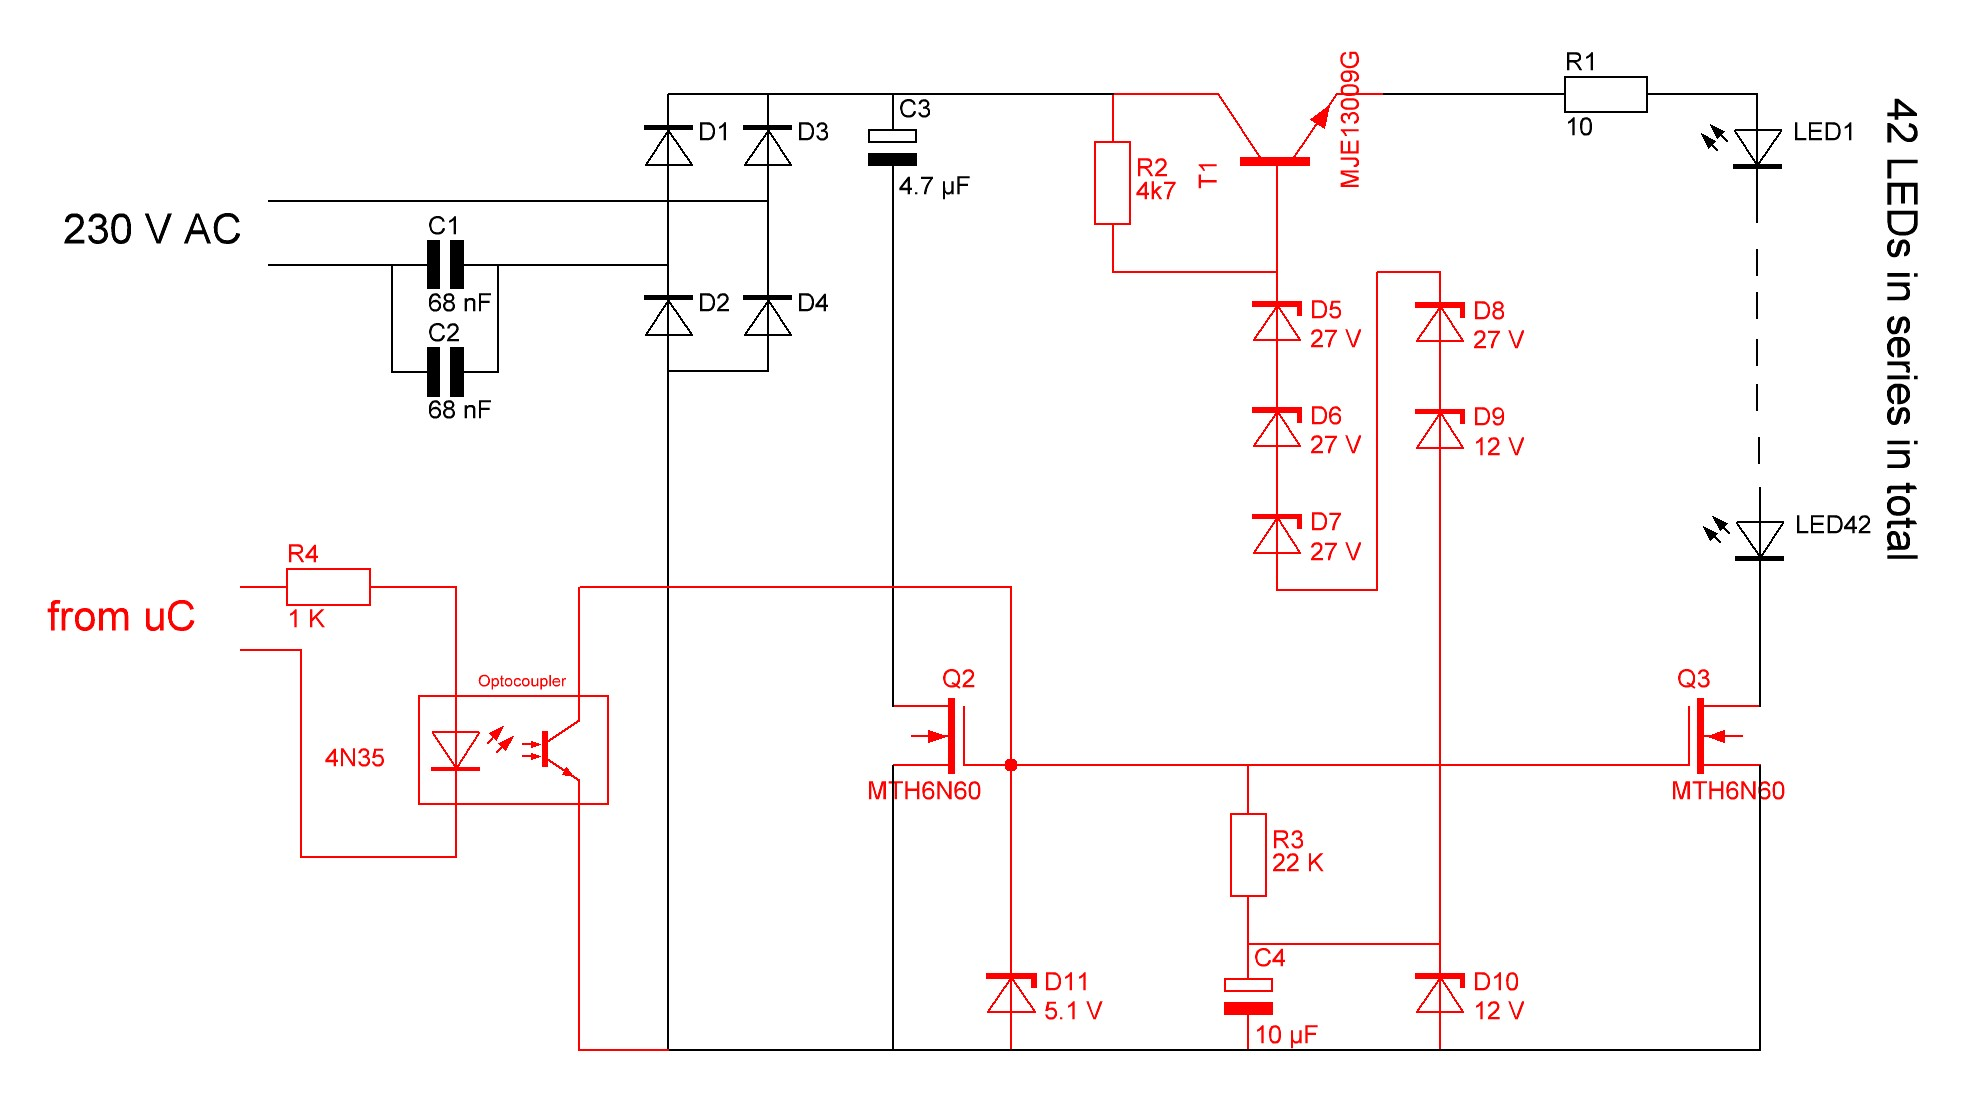
\includegraphics[angle=90,width=\textwidth,height=.9\textheight,keepaspectratio]{chapters/appendix/commercial-230v-ac-modified-schematic/commercial-230v-ac-modified-schematic.jpg}
	\caption{Schematic of the modified commercial 230 V AC LED. Everything in black is from the original schematic. Everything in red is added in order to modulate the LED safely with a microprocessor.}
	\label{fig:commercial-230v-ac-modified-schematic}
\end{figure}
